\begin{figure}[ht]
   \centering
   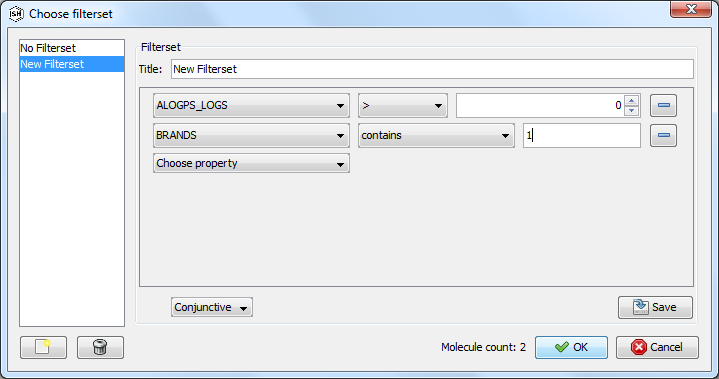
\includegraphics[width=\textwidth]{images/sh_filter_dialog.png}
   \caption{Filter Dialog}
   \label{fig:filter_dialog}
\end{figure}

The \guidialog{Filter Dialog} shown in \figref{fig:filter_dialog} is used to filter the molecules of a dataset, so that you can work with molecules relevant to your problem.
On the left hand side of the dialog a list shows the previously used filtersets.
A filterset is a set of filters.
One filter defines a constraint for one property of the molecules or scaffolds of the dataset.
A combination of filters can be used to filter the dataset by more than one property.
In the lower left corner of the window there are buttons to add a new filterset, or to delete an existing one.
After selecting one of these filtersets, or after creating a new one, the right hand side of the window shows the details of the selected filterset.
Here the title can be changed and filters can be added or modified.
To add a new filter, simply select a property from the \gui{Choose property} box.
For this property, the user can then select a constraint in the appearing drop-down box.
For numerical properties, this box holds comparison operators like ``greater'' ({$>$}) or ``equal'' ($=$).
For text properties, the user can select comparison operators like ``contains'' or ``ends with''.
Both property types can also be filtered by whether or not they are defined.
With the ``minus'' button at the end of each row, the corresponding filter can be removed.
With the \gui{conjunctive / disjunctive} box you can define the operator used to combine the filters.
With the conjunctive method, all filters have to match to allow a molecule to be added to the resulting dataset.
With the disjunctive method, only one filter needs to match.

The \gui{Save} button simply saves the changes made to the selected filterset.
To use a filterset, select it and click the \gui{Ok} button.
If the filterset was not saved before clicking \gui{Ok} and you continue without saving, the current filterset is used for filtering, but the changes are discarded afterwards.
